\documentclass[reprint,aps,pra,floatfix,superscriptaddress,longbibliography,nofootinbib]{revtex4-2}

\usepackage[T1]{fontenc}
\usepackage{newtxtext}
\usepackage{newtxmath}
\usepackage{graphicx}
\usepackage{booktabs}
\usepackage{array}
\usepackage{amsmath}
\usepackage{microtype}
\usepackage{xcolor}
\usepackage[colorlinks=true,linkcolor=black,citecolor=black,urlcolor=black]{hyperref}

\newcommand{\dEz}{\Delta E_z}
\newcommand{\Ts}{T_2^{*}}
\newcommand{\ee}[2]{#1\times10^{#2}}
\newcommand{\fa}{\textsuperscript{a}}
\newcommand{\fd}{\textsuperscript{d}}
\newcommand{\fb}{\textsuperscript{b}}
\newcommand{\ff}{\textsuperscript{f}}

\begin{document}

\title{Error budgets for exchange-based two-qubit gates in four published silicon spin-qubit devices}

\author{Jasper Sands}

\date{October 2026}

\begin{abstract}
We compare the measured two-qubit gate fidelities of four published silicon spin-qubit devices (Xue \emph{et al.}\ 2022, Noiri \emph{et al.}\ 2022, Mills \emph{et al.}\ 2022 and device A of Tanttu \emph{et al.}\ 2024) with a first-order error budget of an exchange-pulsed CZ gate that contains only the noise each paper characterises. The budget has four parts: the coherent error of the noiseless pulse, Zeeman noise on each qubit, exchange (charge) noise, and Markovian relaxation and dephasing. The Zeeman spectrum is a power law pinned to the measured $\Ts$ and, where a Hahn-echo time is reported, fitted to it. Every input is taken from the papers, and derived, bounded and assumed values are flagged. At the published gate times the model gives infidelities of $\ee{1.35}{-4}$ to $\ee{1.66}{-3}$, which account for 4\,\% (Xue) to 21\,\% (Mills) of the measured error; for Mills the model lies inside the experimental error bar. Quasi-static Zeeman noise is the largest modelled term in all four devices. We then add, one at a time, mechanisms that the papers name but that the base budget leaves out. Those whose inputs are published close 7.9\,\% of the remaining gap for Xue, at most 12.7\,\% for Tanttu, and none of it for Noiri and Mills. For each mechanism with an unpublished input we give the input value that would close the gap on its own. The note contains no new measurements; it puts existing, partial error budgets on a common and reproducible footing.
\end{abstract}

\maketitle

%---------------------------------------------------------------------------
\section{Introduction}
\label{sec:intro}

Two-qubit gates between electron spins in silicon quantum dots now reach average fidelities near or above 99\,\% in several laboratories~\cite{xue2022,noiri2022,mills2022,tanttu2024}. The same papers characterise the noise acting on the qubits: Ramsey and Hahn-echo times, sometimes a fitted charge-noise amplitude, relaxation times and electron temperatures. They report the gate fidelity from interleaved randomized benchmarking (IRB)~\cite{magesan2011,magesan2012} or gate set tomography (GST)~\cite{blumekohout2017,nielsen2021}.

Comparing the two is useful for a simple reason. If the characterised noise accounts for the measured error, the route to better gates runs through that noise: lower charge noise, faster gates, better isotopic purification. If it does not, a large part of the error comes from processes that the coherence measurements do not see, such as drift over the hours a benchmark takes, calibration errors, crosstalk or leakage, and the benchmark number is a statement about the whole control stack rather than about the qubit's environment.

This comparison has been made before, one device at a time, and the models have fallen short. Xue \emph{et al.}\ simulate their CZ with the noise fitted to Ramsey data and obtain $\ee{2.2}{-4}$ against a measured $\ee{3.5}{-3}$, about 6\,\%, and attribute the difference to slower barrier drift~\cite{xue2022}. Noiri \emph{et al.}\ simulate randomized benchmarking with quasi-static noise taken from measured frequency traces and find about 0.1\,\% from dephasing against 0.49\,\% measured, about 20\,\%, and point to pulse calibration errors and long-term fluctuations~\cite{noiri2022}; a later analysis of the same gate identifies coherent phase errors in the CROT~\cite{wu2024}. Mills \emph{et al.}\ name charge noise as a likely limit without a numerical budget~\cite{mills2022}. Tanttu \emph{et al.}\ use GST to decompose the error of gates on three devices into stochastic and Hamiltonian generators, follow its variation in lab time, and report errors that their identified mechanisms do not fully explain~\cite{tanttu2024}. The closest prior work is Rimbach-Russ \emph{et al.}~\cite{rimbachruss2023}, who compare simulated and measured two-qubit errors for the Xue and Mills devices, find the simulations below the measurements, and stress coherent control errors and heating as candidates; heating-induced shifts of the qubit frequencies are documented separately~\cite{undseth2023}. A recent shuttling-based experiment again reports a noise model that accounts for roughly a fifth of the measured two-qubit error~\cite{matsumoto2026}. Exchange-only qubits are a contrast: there the error model of Weinstein \emph{et al.}\ is reported to be consistent with the measured data~\cite{weinstein2023}. Reviews state that two-qubit fidelities in silicon are limited mainly by charge and magnetic noise~\cite{burkard2023}.

Each of these analyses uses its own model, its own noise inputs and its own definition of the gate. To our knowledge no prior work applies one noise model, with parameters sourced from each paper, to several published silicon devices and reports the fraction of the measured error it explains. This note does that for four devices. The underprediction it finds is not new for any single device, and its per-device numbers agree in size with the estimates above; the contribution is narrow: a uniform error budget in which every input is traced to a table, figure or section of the source paper, a statement of which inputs had to be assumed, and the code that reproduces every number~\cite{code}. It does not add measurements, and it does not establish which mechanism causes the remaining error; it shows how large that remainder is under the stated assumptions, and what size the candidate mechanisms would need to have to account for it.

%---------------------------------------------------------------------------
\section{Model}
\label{sec:model}

\subsection{Gate}

Two electron spins, in the frame rotating at the mean Zeeman frequency, evolve under
\begin{equation}
\frac{H(t)}{h} = \frac{J(t)}{4}\left(X_1X_2+Y_1Y_2+Z_1Z_2\right) + \frac{\Delta B_z}{2}\left(Z_1-Z_2\right),
\label{eq:H}
\end{equation}
where $J(t)$ is the exchange and $\dEz = 2\Delta B_z$ is the difference of the qubit frequencies, the quantity the device papers quote. Frequencies are in MHz and times in ns. For $\dEz \gg J$ an exchange pulse produces a conditional phase $2\pi\cdot10^{-3}\int J\,dt$ for any pulse shape, so a CZ requires an area of $500$\,MHz\,ns; the single-qubit $Z$ phases that come with it are removed by virtual-$Z$ frame updates. Each device is modelled with a window close to its published pulse: a cosine (Hann) window for Xue, a Tukey window with 4\,ns cosine edges for Mills, and a square pulse for Tanttu. Noiri's gate is a CNOT made of two controlled rotations (CROT) under always-on exchange; there the model asks what a cosine-window CZ of the same duration would give in the same noise, and the two gates are not the same (Sec.~\ref{sec:devices}).

\subsection{Four error contributions}

The infidelity of the pulse is split into four parts, all reported as average gate infidelities $1-F_\mathrm{avg} = \tfrac{d}{d+1}(1-F_e)$ with $d=4$, the quantity RB and GST estimate~\cite{magesan2011,nielsen2021}.

(a) Coherent error: the exact noiseless propagator, compared with a CZ after the best virtual-$Z$ correction. For smooth windows this is the non-adiabatic transfer between $|{\uparrow\downarrow}\rangle$ and $|{\downarrow\uparrow}\rangle$; a square pulse has none at the synchronised times $T_n=\sqrt{n^2-1/4}\,/\dEz$.

(b) Zeeman noise on each qubit frequency, with noise operator $Z_q/2$. The quasi-static part has the Gaussian width $\sigma_q = \sqrt{2}/(2\pi\Ts)$ that a Ramsey experiment measures (for Xue the reported widths of 11 and 24\,kHz are used directly).

(c) Exchange noise $\delta J(t) = J(t)\,\eta(t)$, with noise operator $(\boldsymbol{\sigma}_1\cdot\boldsymbol{\sigma}_2)/4$ and $\eta$ of quasi-static width $\sigma_J$, the relative exchange noise $\delta J/J$.

(d) Markovian relaxation and dephasing from the Lindblad equation, with $T_1$ per qubit, detailed balance at the electron temperature, and white dephasing only where the echo decay requires it (below).

Terms (b) and (c) are computed with toggle-frame filter functions~\cite{green2013,hangleiter2021}. For a noise source with operator $N_\alpha$ and sensitivity $a_\alpha(t)$ the control matrix is $R_{\alpha\beta}(\omega) = \int_0^T dt\, e^{i\omega t} a_\alpha(t)\, \mathrm{Tr}[C_\beta U_0^\dagger(t) N_\alpha U_0(t)]$, with $C_\beta$ the two-qubit Pauli basis and $U_0$ the noiseless propagator, evaluated in closed form within each piecewise-constant slice. With $F_\alpha(\omega) = \sum_\beta |R_{\alpha\beta}(\omega)|^2$ the entanglement infidelity to first order is
\begin{equation}
1-F_e \simeq \frac{1}{d}\sum_\alpha\left[\sigma_\alpha^2 F_\alpha(0) + \int_{\omega_R}^{\infty} \frac{d\omega}{2\pi}\, S_\alpha(\omega) F_\alpha(\omega)\right],
\label{eq:ff}
\end{equation}
where the first term is the quasi-static noise within the Ramsey band and the second the noise above it, with $\omega_R = 2\pi/\Ts$ ($\Ts$ averaged over the two qubits).

\subsection{Spectra pinned to $\Ts$ and fitted to the echo}

Charge noise in silicon devices has an approximately $1/f$ spectrum~\cite{paladino2014,yoneda2018,connors2022}. The model takes $S_q(f) = A_q f^{-\alpha_q}$ for each qubit frequency and fixes $A_q$ so that the integral over the Ramsey band, from $1/\tau_\mathrm{avg}$ (one over the Ramsey averaging time) to $1/\Ts$, equals $\sigma_q^2$. The quasi-static term of Eq.~\eqref{eq:ff} and the spectrum above the band are then the same noise, not two independent inputs. The same spectrum predicts a Hahn-echo decay $\exp[-(t/T_2)^{\alpha+1}]$ with
\begin{equation}
T_2 = \frac{2}{\pi}\left[8 A\, I(\alpha)\right]^{-1/(\alpha+1)}, \quad I(\alpha) = \int_0^\infty x^{-\alpha-2}\sin^4 x\,dx,
\end{equation}
with $I(1)=\ln 2$~\cite{cywinski2008}. Where a paper reports an echo time, $\alpha_q$ is fitted per qubit, within $0.5\le\alpha\le2.5$, so that the pinned spectrum reproduces it. Where the echo is shorter than any allowed spectrum predicts, the shortfall is read as white dephasing and enters term (d); otherwise term (d) contains no dephasing, so that low-frequency noise is not counted twice. Xue \emph{et al.}\ report no echo time, and there $\alpha=1$. The exchange noise has $\alpha=1$ for every device, since none of the papers gives an exchange-noise spectrum, and is pinned to $\sigma_J$ over the same band.

\subsection{Assumptions and checks}

The budget is first order in the noise, and the four parts are added. The Zeeman and exchange noises are taken to be independent; the noise is Gaussian and stationary; the gate is isolated, with no single-qubit gates, idles, crosstalk or leakage to other states. The package tests check that the four parts agree within about 5\,\% with one Lindblad simulation in which all noise acts at once (quadrature over the quasi-static offsets, Monte Carlo over the fast traces), for each of the four devices; that the closed-form echo time agrees with numerical integration of the echo filter function; and that each device's fitted spectrum returns its reported $\Ts$ and echo times within 6\,\%~\cite{code}.

%---------------------------------------------------------------------------
\section{Devices and parameters}
\label{sec:devices}

\begin{table*}
\caption{Model inputs. Per-qubit values are listed Q1, Q2. Unmarked values are printed in the cited version of the paper; \fd\ derived from reported numbers, \fb\ upper bound, \fa\ assumed, \ff\ fitted by the model. Every value, with its source and the reason for each flag, is in \texttt{data/devices.json} of Ref.~\onlinecite{code}.}
\label{tab:params}
\small
\begin{ruledtabular}
\begin{tabular}{lllll}
 & Xue 2022~\cite{xue2022} & Noiri 2022~\cite{noiri2022} & Mills 2022~\cite{mills2022} & Tanttu 2024, device A~\cite{tanttu2024} \\
\midrule
Platform & $^{28}$Si/SiGe, micromagnet & $^{28}$Si/SiGe, micromagnet & $^{28}$Si/SiGe, micromagnet & SiMOS, $g$-factor difference \\
Values read from & published version & arXiv v2 & published version & arXiv v3 \\
Measured gate, method & CZ, GST & CNOT (two CROT), IRB & CZ, IRB & CZ, IRB \\
Measured fidelity (\%) & $99.65\pm0.15$ ($2\sigma$) & $99.51\pm0.02$ & $99.81\pm0.17$ & $98.42\pm0.22$ \\
Gate time (ns) & 100 & 103 & 40 & 256 \\
$\dEz$ (MHz) & 103\fd & 300 & 396\fd & 10.8 idle, 11.555\fa\ in pulse \\
$J$ reported for the gate (MHz) & 10.06 & 18.85 (always on) & 12.5 & 1.95 \\
Peak $J$ of the model pulse (MHz) & 10.0 & 9.7 & 13.9 & 1.95 \\
Exchange ceiling (MHz) & 20 & 32.0 & 13.9, the model's peak & 1.95\fa \\
Model window & cosine & cosine\fa & Tukey, 4\,ns edges\fa & square \\
$\Ts$ ($\mu$s) & 20.5, 9.4\fd & 7.05, 7.3\fd & 1.7, 2.3 & 5.5, 6.5 \\
Hahn-echo $T_2$ ($\mu$s) & not reported & 31.6, 29.7\fd & 23, 102 & 51, 60 \\
Zeeman exponent $\alpha$ & 1\fa & 0.97, 0.94\ff & 1.23, 1.50\ff & 1.17, 1.17\ff \\
$T_1$ (ms) & 10\fa & 10\fa & 24, 18 & 10\fa \\
Quasi-static $\delta J/J$ & 0.97\,\%\fd & 0.34\,\%\fb & 0.97\,\%\fa\ (Xue's) & 1.6\,\%\fa \\
Electron temperature (mK) & 55\fa & 60 & 45 & 100\fa \\
Ramsey averaging time (s) & 480 & 87 & 100\fa & 100\fa \\
\end{tabular}
\end{ruledtabular}
\end{table*}

Table~\ref{tab:params} lists the inputs. The four devices differ in ways that matter for the comparison.

Xue 2022~\cite{xue2022}. The exchange is controlled by a barrier gate, with $J(v_B) = J_\mathrm{res}e^{2\alpha v_B}$, and the CZ is a cosine window in $J$ of 100\,ns. The quasi-static widths of the qubit frequencies (11 and 24\,kHz) and of the barrier voltage (0.4\,mV) are fitted to Ramsey data averaged for about 8 minutes; $\delta J/J = 0.97\,\%$ follows from the barrier noise and the exchange lever arm. $T_1$ and the electron temperature are not reported; the temperature is taken from a similar device~\cite{xue2021}, and neither matters at 100\,ns.

Noiri 2022~\cite{noiri2022}. The exchange is always on and the CNOT consists of two resonantly driven CROT pulses. The model's cosine CZ of 103\,ns needs a peak of only 9.7\,MHz. The paper states that the single-qubit frequency noise exceeds the exchange noise $\Delta J/2$; taking the frequency noise to be at most the conditional Ramsey width of Q1 (31.9\,kHz) bounds $\delta J/J$ below 0.34\,\%, and that bound is used. The exchange term is only $\ee{7}{-6}$ with it.

Mills 2022~\cite{mills2022}. The CZ is a 40\,ns barrier pulse smoothed with a binomial filter; the published version gives $J\approx12.5$\,MHz (arXiv v1 gives about 5\,MHz). A Tukey window with the same peak reaches only 450\,MHz\,ns, so the model raises the peak to 13.9\,MHz. No exchange-noise amplitude is reported, and Xue's is used.

Tanttu 2024, device A~\cite{tanttu2024}. The CZ is a 256\,ns square exchange pulse on a SiMOS device without a micromagnet. At the idle $\dEz=10.8$\,MHz this pulse is not synchronised and would leave a SWAP-like coherent error of $\ee{4.0}{-3}$, which the paper's GST error channels for this CZ do not show. The exchange-gate pulse Stark-shifts the qubits and its voltage is fed back during the run, so the model assumes that $\dEz$ during the pulse is the nearest synchronised value, 11.555\,MHz ($n=3$), and reports the idle-value error separately. The exchange noise combines Xue's 0.4\,mV gate noise with this device's exchange slope of 17.13 decades per volt.

%---------------------------------------------------------------------------
\section{Results}
\label{sec:results}

\begin{table}
\caption{Measured and modelled average gate infidelity at the published gate time, in units of $10^{-4}$. The coherent term is below $10^{-6}$ for every device; for Tanttu it would be 40 at the idle $\dEz$. The last column is the model total as a share of the measured infidelity.}
\label{tab:results}
\begin{ruledtabular}
\begin{tabular}{lrrrrrr}
 & measured & model & Zeeman & exchange & Markov. & share \\
\midrule
Xue & $35\pm15$ & 1.35 & 0.68 & 0.59 & 0.080 & 3.9\,\% \\
Noiri & $49\pm2$ & 2.33 & 2.17 & 0.071 & 0.082 & 4.7\,\% \\
Mills & $19\pm17$ & 4.00 & 3.44 & 0.55 & 0.016 & 21\,\% \\
Tanttu A & $158\pm22$ & 16.6 & 14.9 & 1.50 & 0.20 & 10.5\,\% \\
\end{tabular}
\end{ruledtabular}
\end{table}

\begin{figure*}
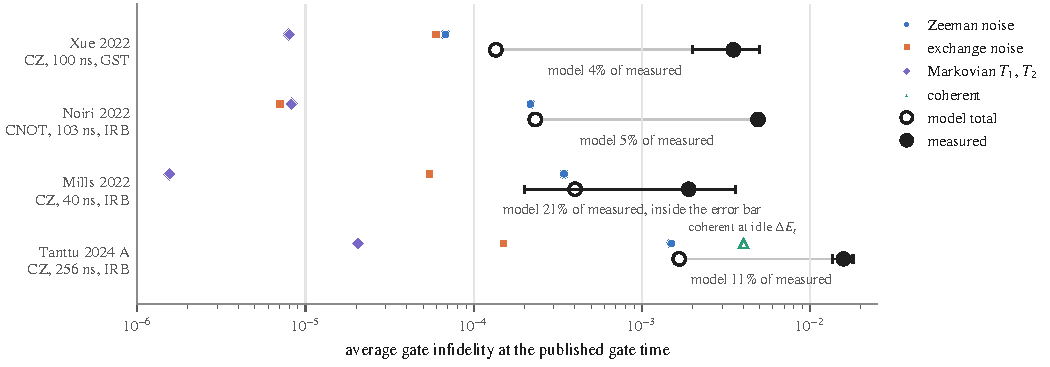
\includegraphics[width=\textwidth]{figures/summary.pdf}
\caption{Modelled error contributions (small markers, offset upwards), model total (open circle) and measured infidelity (filled circle, with the reported uncertainty) at the published gate time of each device. For Tanttu the open triangle is the coherent error the square pulse would have at the idle $\dEz=10.8$\,MHz instead of the assumed 11.555\,MHz.}
\label{fig:summary}
\end{figure*}

Table~\ref{tab:results} and Fig.~\ref{fig:summary} give the comparison. The modelled fidelities are 99.986\,\% (Xue), 99.977\,\% (Noiri), 99.960\,\% (Mills) and 99.834\,\% (Tanttu). The measured error is 26, 21, 4.7 and 9.5 times the modelled one, so the characterised noise accounts for 4\,\% (Xue) to 21\,\% (Mills) of it. Only for Mills does the model lie inside the reported uncertainty, which is $\pm0.17\,\%$.

Zeeman noise is the largest modelled term in all four devices, with exchange noise close behind for Xue. Most of the budget is quasi-static: the quasi-static parts of the Zeeman and exchange terms are $\ee{1.02}{-4}$ of $\ee{1.35}{-4}$ for Xue, $\ee{1.71}{-4}$ of $\ee{2.33}{-4}$ for Noiri, $\ee{3.89}{-4}$ of $\ee{4.00}{-4}$ for Mills and $\ee{1.60}{-3}$ of $\ee{1.66}{-3}$ for Tanttu. For a given spectrum the budget is therefore set mainly by the quasi-static widths behind $\Ts$ and by the gate time; the exception is the white dephasing that the echo fit can introduce, discussed next. Relaxation contributes less than $\ee{3}{-5}$ everywhere, and the coherent error of the modelled windows is negligible.

The fitted exponents are 0.97 and 0.94 for Noiri, 1.23 and 1.50 for Mills, and 1.17 for both Tanttu qubits. With $\alpha=1$ on every qubit instead, Mills would be $\ee{4.6}{-4}$ and Tanttu $\ee{1.8}{-3}$: their echoes are longer than $1/f$ predicts, so the fit places less noise above the Ramsey band. Noiri moves most, from $\ee{2.3}{-4}$ to $\ee{8.2}{-4}$; with $\alpha=1$ its echoes come out slightly shorter than predicted and the shortfall is read as white dephasing, which then dominates. The Noiri total is $\ee{2.6}{-4}$ at $\alpha=0.9$ and $\ee{1.9}{-3}$ at $\alpha=1.1$, so its budget is the least certain of the four. Mills and Tanttu do not report a Ramsey averaging time; between 10\,s and 1\,h the totals move by less than 0.4\,\%, but the fitted exponents move from 1.63 to 1.37 (Mills Q2) and from 1.23 to 1.12 (Tanttu).

\begin{figure}
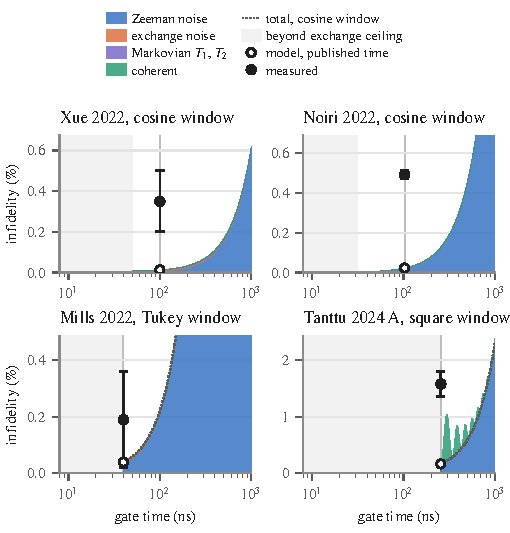
\includegraphics[width=\columnwidth]{figures/budget_vs_time.pdf}
\caption{Modelled infidelity against gate time, stacked by contribution, for the window used for each device. Grey: gate times that need more exchange than the ceiling of Table~\ref{tab:params}. For Mills and Tanttu the dotted line is the total for a cosine window. The square pulse for Tanttu has coherent error between its synchronised times.}
\label{fig:time}
\end{figure}

Figure~\ref{fig:time} shows the budget as a function of gate time. The noise terms keep falling as the gate gets shorter, so under the largest exchange each paper shows, the lowest modelled error sits at or near the exchange ceiling: a square pulse at a synchronised time gives 99.9927\,\% at 28.7\,ns for Xue, 99.9985\,\% at 16.6\,ns for Noiri and 99.9636\,\% at 37.9\,ns for Mills, and for Tanttu the published 256\,ns is already the shortest time the reported exchange allows. The comparison in Table~\ref{tab:results} is made at the published gate times, not at these optima.

%---------------------------------------------------------------------------
\section{Candidate mechanisms for the gap}
\label{sec:gap}

The papers' own error analyses name mechanisms beyond the noise in the base budget. We add them as separate first-order terms, each switched on only when its input is given, and report what each closes of the gap, defined as measured minus modelled infidelity. Where an input is published, or follows from published numbers, the term is evaluated; where it is not, it is computed as a function of that input, and we give the value that would close the gap on its own.

Qubit frequencies moved by the exchange-gate voltage. Xue \emph{et al.}\ fit $f_j(v_B) = f_j(0) + \beta_j v_B^{\gamma}$ ($\beta_1=-2.91$ and $\beta_2=67.2$\,MHz\,V$^{-\gamma}$, $\gamma=1.20$). If the exchange noise is noise on that voltage, it also shifts the qubit frequencies, correlated with $\delta J$; the term adds that shift to the exchange-noise source in the filter function. Where no fit is published, it is parametrised by $df/d\ln J$ of one qubit.

Noise slower than the Ramsey average. The fitted spectra are extended from $1/\tau_\mathrm{avg}$ down to one over the time the benchmark runs without recalibrating that quantity, and the added variance is treated as quasi-static within a gate.

Pulse distortion. A single-pole low-pass filters the gate voltage (mapped to $J$ with the paper's $J(v)$ for Xue and Tanttu, or $J$ directly for Mills), and the pulse area is recalibrated to the CZ, as the experiments recalibrate the exchange.

Residual exchange outside pulse adds a conditional phase $\phi=2\pi\cdot10^{-3}\int J\,dt$ and, after the best virtual-$Z$ correction, an infidelity $\tfrac{4}{5}\sin^2(\phi/4)$.

Uncalibrated offsets of the qubit frequencies or of $J$ during the gate (drift between recalibrations, shifts after microwave bursts or exchange pulses, calibration errors) enter like quasi-static noise of the same rms size, so the required offset can be compared directly with the fitted quasi-static width.

The coherent residual that GST measures for Xue's CZ, $\tfrac45\theta_J^2$ with $\theta_J=0.016$, is added as measured.

\begin{table*}
\caption{What each candidate mechanism adds, with its share of the gap in parentheses, or the input value that would close the gap on its own. (d) derived from published numbers: Xue's GST run of about 4\,h from the recalibration schedule, Tanttu's IRB run of 2.2\,h from 200 batches of about 40\,s. ``Upper bound'' ($\le$): the quantity was fed back during the run. $^\dagger$Shift of one qubit frequency per e-fold change of $J$, $df/d\ln J$. Frequency offsets are compared with the fitted quasi-static widths (kHz), exchange offsets with the quasi-static $\delta J/J$.}
\label{tab:gap}
\footnotesize\setlength{\tabcolsep}{3pt}
\begin{tabular}{@{}>{\raggedright}p{3.95cm}>{\raggedright}p{3.2cm}>{\raggedright}p{3.05cm}>{\raggedright}p{3.3cm}>{\raggedright\arraybackslash}p{3.4cm}@{}}
\hline\hline\noalign{\vskip 2pt}
Mechanism & Xue 2022 & Noiri 2022 & Mills 2022 & Tanttu 2024 A \\
\noalign{\vskip 1pt}\hline\noalign{\vskip 2pt}
Gap (measured $-$ model) & $\ee{3.36}{-3}$ & $\ee{4.67}{-3}$ & $\ee{1.50}{-3}$, inside error bar & $\ee{1.41}{-2}$; $\ee{3.0}{-2}$ vs.\ GST \\
Gate voltage moves qubit frequencies & $\ee{3.6}{-5}$ (1.1\,\%) & no exchange pulse & not closed below 30\,MHz$^\dagger$ & needs 10\,MHz$^\dagger$ \\
Zeeman noise below Ramsey band & $\ee{8.6}{-6}$ (0.3\,\%), 2\,h & 1.3\,\% even at 1000\,h & closes it at about 2.8\,h & $\le\ee{1.75}{-3}$ (12\,\%), 2.2\,h\fd \\
Exchange noise below Ramsey band & $\ee{1.5}{-5}$ (0.4\,\%), 4\,h\fd & 0.1\,\% at 1000\,h & 1.8\,\% at 1000\,h & $\le\ee{3.4}{-5}$ (0.2\,\%) \\
Pulse distortion (bandwidth) & $<0.1$\,\% down to 1\,MHz & does not apply & lowers the error & needs $\le2.7$\,MHz \\
Residual exchange outside pulse & needs 41\,MHz\,ns per CZ & does not apply & needs 28\,MHz\,ns & needs 85\,MHz\,ns \\
Frequency offset needed (rms) & 146\,kHz (widths 11, 24) & 167\,kHz (32, 31) & 244\,kHz (132, 98) & 118\,kHz (41, 35) \\
Exchange offset needed (rms $\delta J/J$) & 8.2\,\% (width 0.97\,\%) & 9.7\,\% (bound 0.34\,\%) & 5.5\,\% (assumed 0.97\,\%) & 16.5\,\% (assumed 1.6\,\%) \\
Coherent residual measured by GST & $\ee{2.05}{-4}$ (6.1\,\%) & no GST of the gate & no GST of the CZ & not tabulated \\
Heating or leakage during drive & no number & $\le\ee{1.6}{-3}$ (34\,\%), not modelled & no number & plotted only \\
\noalign{\vskip 1pt}\hline\noalign{\vskip 2pt}
Closed by published-input terms & 7.9\,\% & 0 & 0 & 12.7\,\%, an upper bound \\
\noalign{\vskip 1pt}\hline\hline
\end{tabular}
\end{table*}

\begin{figure*}
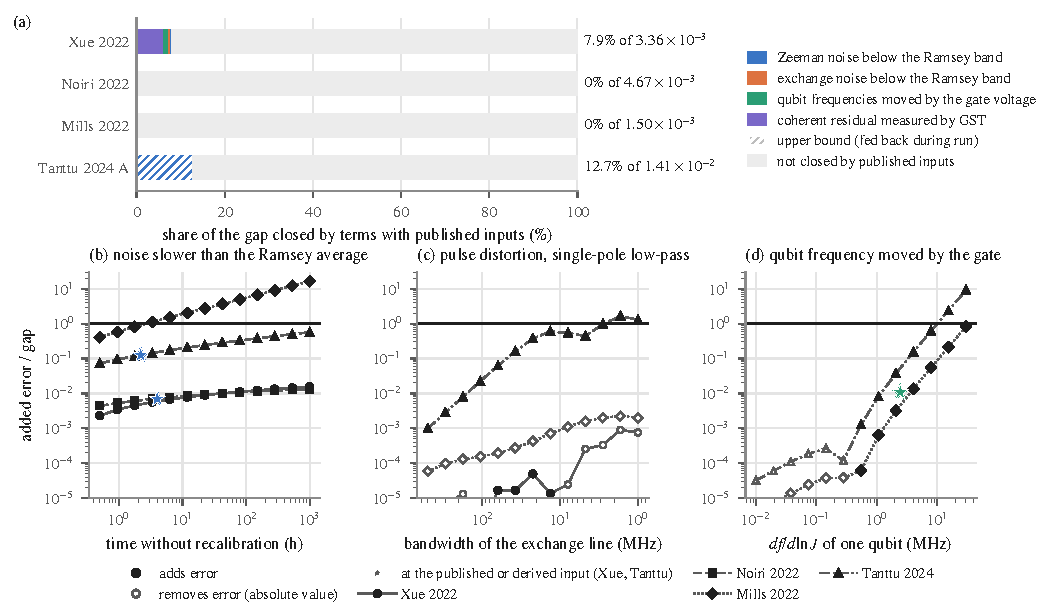
\includegraphics[width=\textwidth]{figures/gap_mechanisms.pdf}
\caption{(a) Share of each device's gap closed by the terms whose inputs are published. Hatched: an upper bound, because the quantity was fed back during the run. (b)--(d) Terms whose input is not published, divided by each gap, as a function of that input; the horizontal line marks where the term alone closes the gap. Open markers: the term lowers the error (absolute value shown). Stars: the value at the published or derived input. In (b) the Zeeman and exchange terms are summed.}
\label{fig:gap}
\end{figure*}

Table~\ref{tab:gap} and Fig.~\ref{fig:gap} summarise the result.

Xue 2022. The terms with published inputs add $\ee{2.7}{-4}$, 7.9\,\% of the gap, and three quarters of that is the coherent part that GST itself measures. With the barrier coupling of the qubit frequencies the model gives $\ee{1.72}{-4}$, close to the authors' own simulation of $\ee{2.2}{-4}$, which includes the same coupling; with every published term it gives $\ee{4.0}{-4}$. The remaining $\ee{3.1}{-3}$ is stochastic according to GST. On its own it would require an rms exchange error of 8.2\,\% during the gate, eight times the width fitted from 8-minute Ramsey data, or qubit-frequency offsets of 146\,kHz rms, six to thirteen times the fitted widths. Extending the fitted $1/f$ spectrum over the whole 4\,h run adds only $\ee{1.5}{-5}$, so the barrier drift the authors propose would have to grow much faster toward low frequencies than $1/f$. A random-walk drift of $J$ that adds the whole gap at the paper's 2\,h recalibration interval would be about 8\,\%/$\sqrt{\mathrm{h}}$, and would require recalibrating $J$ every 25 minutes to hold 99.9\,\%; this is a reading of the authors' attribution, not a measured rate.

Noiri 2022. No term with published inputs applies, because the measured gate has no exchange pulse. The slow-noise terms grow only logarithmically for $\alpha$ near 1 and reach 1.3\,\% of the gap at 1000\,h. The authors' own accounting is about $\ee{1}{-3}$ from dephasing, from their simulation with 4.7\,h of measured noise traces, and at most $\ee{1.6}{-3}$ from drive-related errors, bounded by the single-qubit primitive, which is also two CROT pulses. The model's quasi-static terms give $\ee{1.7}{-4}$ for the CZ, six times less than their dephasing estimate; the gates differ (in a CROT, frequency noise also detunes the drive, and the pulsed CZ has no drive), and their traces, recorded over hours, include drift slower than the 87\,s Ramsey average. That leaves at least $\ee{2.3}{-3}$ for what the authors call pulse calibration errors and long-term fluctuations; Wu \emph{et al.}\ identify coherent phase errors of the CROT as one such contribution~\cite{wu2024}, which a pulsed-CZ model cannot represent.

Mills 2022. The model is already inside the $\pm\ee{1.7}{-3}$ error bar. If the benchmark ran for about 2.8\,h without recalibration, the fitted Zeeman spectra extended to that time would close the rest; this relies on the fitted exponents holding below 10\,mHz and on the assumed 100\,s Ramsey averaging, and neither the run time nor the averaging time is published.

Tanttu 2024, device A. Slow Zeeman noise over the 2.2\,h run gives the largest published-input term, at most $\ee{1.75}{-3}$ (12\,\%); the qubit frequencies were fed back during the run, which removes part of it. A line bandwidth of 2.7\,MHz or less would close the gap, but through a SWAP-like coherent error that the paper's GST does not show for this CZ. Moving the qubit frequencies through the gate voltage would need 10\,MHz per e-fold of $J$, about 130\,MHz across the 330\,mV swing, against $\dEz=10.8$\,MHz. The remaining $\ee{1.24}{-2}$ (87\,\%), or $\ee{2.9}{-2}$ against GST, is not closed by anything published.

What the benchmarks report also bounds the comparison. IRB returns the gate error exactly only for depolarising errors; otherwise the true error lies within $\pm E$ of the estimate, with $E = 2r_\mathrm{ref}-r_\mathrm{est}$ when the reference Clifford error $r_\mathrm{ref}$ dominates~\cite{magesan2012}. With the published reference Clifford errors of 1.3\,\%, 6.8\,\% and 9.3\,\%, $E$ is $\ee{2.2}{-2}$ for Noiri, 0.13 for Mills and 0.17 for Tanttu, each wider than the gap. The bound is pessimistic when errors are close to depolarising, and it does not mean the reported fidelities are wrong, but IRB alone does not exclude an error as small as the model's. GST separates coherent from stochastic error, but drift during the run appears as stochastic error~\cite{tanttu2024}, so it cannot distinguish slow drift from fast noise.

%---------------------------------------------------------------------------
\section{Discussion and limitations}
\label{sec:discussion}

Under the assumptions stated, the noise that the four papers characterise accounts for 4\,\% to 21\,\% of the measured two-qubit error, and the mechanisms whose inputs are published add little: 7.9\,\% of the gap for Xue, at most 12.7\,\% for Tanttu, and nothing for Noiri and Mills. The per-device fractions are in line with the authors' own estimates where those exist (about 6\,\% for Xue's simulation) and with the two-device comparison of Ref.~\onlinecite{rimbachruss2023}; the larger fraction from Noiri's own simulation (about 20\,\%) comes from a simulation of the CROT gate itself, with noise traces recorded over hours. The candidates that could close the gaps are drift or calibration error of $J$ and of the qubit frequencies at the level of 5.5--16.5\,\% rms in $\delta J/J$ or 118--244\,kHz rms in frequency, slow noise steeper than $1/f$, pulse distortion (for Tanttu), heating of the device during driving~\cite{undseth2023}, and errors outside the isolated gate, none of which the papers quantify for the benchmarked gates. Measuring the benchmark duration, the exchange-line bandwidth, the dependence of the qubit frequencies on the exchange-gate voltage and the low-frequency exchange-noise spectrum would turn several entries of Table~\ref{tab:gap} from required values into evaluated ones.

The comparison has limits that should be read with it.
The model is an estimate, not a bound in either direction: the assumed values, the fitted spectra and the windows can each move it up or down. $T_1$ is assumed for three of the four devices, and only Xue reports an exchange-noise width; Noiri's is an upper bound, and Mills and Tanttu borrow Xue's gate-voltage noise.
The Zeeman exponent rests on two numbers per qubit, $\Ts$ and one echo time, and on a single power law across the band; Noiri's total changes by a factor of about seven between $\alpha=0.9$ and $1.1$.
Noiri's gate is a resonantly driven CROT-based CNOT under always-on exchange ($J=18.85$\,MHz), not an exchange-pulsed CZ; it is modelled as a CZ of the same duration, so for that device the comparison is between a noise environment and a different gate. For Tanttu only device A and its plain CZ are modelled; the decoupled CZ of devices B and C is not.
Mills's interleaved-RB uncertainty of $\pm0.17\,\%$ is almost as large as the measured error, so the 21\,\% explained fraction for that device is poorly constrained.
Zeeman and exchange noise are treated as independent. Where both come from the same charge fluctuators, as Mills \emph{et al.}\ suggest, they are correlated and the sum can be off in either direction.
The gap terms are first order and added one at a time; leakage and microwave crosstalk are not modelled, because no paper gives valley or orbital energies or crosstalk amplitudes.
The measured fidelities are averages over runs of hours and include single-qubit-gate errors only through the IRB reference or the GST gate set; GST and IRB give different values for the same Tanttu gate (96.8\,\% against 98.42\,\%).

%---------------------------------------------------------------------------
\section*{Code availability}

The model, the sourced device parameters, the tests and the scripts behind every number and figure are at \url{https://github.com/Jaspersands/spin-optimal-control}~\cite{code} (version 0.5.0 plus the gap analysis, commit \texttt{d729d58}); the figures here are drawn from its \texttt{figures/comparison.json}.

\bibliography{refs}

\end{document}
